%%%%%%%%%%%%%%%%%%%%%%%%%%%%%%%%%%%%%%%%%%%%%%%%%%%%%%%%%%%%%%%%%%
%%%%%%%% ICML 2016 EXAMPLE LATEX SUBMISSION FILE %%%%%%%%%%%%%%%%%
%%%%%%%%%%%%%%%%%%%%%%%%%%%%%%%%%%%%%%%%%%%%%%%%%%%%%%%%%%%%%%%%%%

% Use the following line _only_ if you're still using LaTeX 2.09.
%\documentstyle[icml2016,epsf,natbib]{article}
% If you rely on Latex2e packages, like most moden people use this:
\documentclass[accepted]{article} % With author names, without line numbers
% \documentclass{article} % without author names, with line numbers

% use Times
\usepackage{times}
% For figures
\usepackage{graphicx} % more modern
%\usepackage{epsfig} % less modern
\usepackage{subfigure} 

% For citations
\usepackage{natbib}

% For algorithms
\usepackage{algorithm}
\usepackage{algorithmic}

% As of 2011, we use the hyperref package to produce hyperlinks in the
% resulting PDF.  If this breaks your system, please commend out the
% following usepackage line and replace \usepackage{icml2016} with
% \usepackage[nohyperref]{icml2016} above.
\usepackage{hyperref}

% Packages hyperref and algorithmic misbehave sometimes.  We can fix
% this with the following command.
\newcommand{\theHalgorithm}{\arabic{algorithm}}

% Employ the following version of the ``usepackage'' statement for
% submitting the draft version of the paper for review.  This will set
% the note in the first column to ``Under review.  Do not distribute.''
\usepackage{icml2016} 

% Employ this version of the ``usepackage'' statement after the paper has
% been accepted, when creating the final version.  This will set the
% note in the first column to ``Proceedings of the...''
%\usepackage[accepted]{icml2016}


% The \icmltitle you define below is probably too long as a header.
% Therefore, a short form for the running title is supplied here:
\icmltitlerunning{Journal 01}
\usepackage[utf8]{inputenc}
\usepackage[T1]{fontenc}
\usepackage[francais]{babel}
\usepackage{amsmath}
\usepackage{amssymb}
\usepackage{tikz}
\usetikzlibrary{arrows,calc,through,backgrounds,matrix,decorations.pathmorphing,decorations.pathreplacing}
\usepackage{xcolor}
\usepackage{lipsum}
\usepackage{cancel}
\usepackage{subfigure}
\usepackage{placeins}
\usepackage{coding}


\newcommand{\TODO}{\par\textcolor{red}{À faire: }}

\begin{document} 

\twocolumn[
\icmltitle{Journal 01}

% It is OKAY to include author information, even for blind
% submissions: the style file will automatically remove it for you
% unless you've provided the [accepted] option to the icml2016
% package.
\icmlauthor{Estrade Victor}{victor.estrade@u-psud.fr}
\icmladdress{Université Paris Saclay,\newline
            Espace Technologique, Bat. Discovery - RD 128 - 2e ét., 91190 Saint-Aubin France}
% \icmlauthor{Binome}{email@coauthordomain.edu}
% \icmladdress{Their Fantastic Institute,
%             27182 Exp St., Toronto, ON M6H 2T1 CANADA}

% You may provide any keywords that you 
% find helpful for describing your paper; these are used to populate 
% the "keywords" metadata in the PDF but will not be shown in the document
\icmlkeywords{machine learning, deep learning}

\vskip 0.3in
]

\begin{abstract} 
L'abstract.
\end{abstract}

\section{Le problème} % (fold)
\label{sec:le_probleme}
\TODO Que mettre ici ?

\TODO Expliquer le problème

\subsection{Applications} % (fold)
\label{sub:applications}

% subsection applications (end)

% section le_problème (end)
\section{Le DANN} % (fold)
\label{sec:le_DANN}
Ici vont être résumé les idées principales de \cite{Ganin15}.

\subsection{Rappel sur l'adaptation de domaine} % (fold)
\label{sub:rappel}

L'adaptation de domaine consiste à adapter un modèle entraîné sur certaines
données pour une utilisation sur des données similaires.
Ces nouvelles données sont suffisamment différentes pour endommager les 
performances du modèle. L'adaptation de domaine vise donc à réduire au mieux
cette perte de performance.

On sépare donc les domaines en un domaine Source $D_S$ et un ou plusieurs domaines 
Cibles $D_T$. On cherche à réduire le risque sur le/les domaine(s) Cible(s) $R_{D_T}$.

De plus on ne dispose pas de données annotées dans le domaine Cible. Il nous faut
nous contenter de celles du domaine Source. Cependant la tâche reste exactement la
même, seule la distribution change.

On a donc un seul problème mais les données sont 
tirées de diverses distributions plus ou moins différentes desquelles le modèle
doit extraire les informations pertinentes afin de résoudre le problème.

Selon \cite{BenDavid} le risque sur le domaine Cible est majoré par:
$$ R_{D_T} \le R_{D_S} + \mathcal{H}\text{-divergence}(S,T) + \beta + C $$

où $\beta$ est un terme lié à la capacité de la classe de modèle $\mathcal{H}$
à être efficace sur les deux distributions et $C$ est un terme principalement
lié à la VC-dimension et à la quantité de donnée disponnible.

C'est la $\mathcal{H}\text{-divergence}$ qui va nous intéresser ici.
Il s'agit d'une mesure de la distance entre le domaine Source et Cible.
$\mathcal{H}\text{-divergence}$ est la capacité du meilleur modèle 
$\eta^*\in\mathcal{H}$ à séparer les éléments du domaine Source $D_S$ et du
domaine Cible $D_T$. Autrement dit la capacité de $\eta^*$ à classifier les 
données selon leur origine.

On a donc deux problèmes distincts sur les même données. L'un est le problème que 
l'on cherche à résoudre, ie construire un modèle $h: x \in D^X \mapsto y \in D^Y$
qui trouvera les labels $y$ en fonction des données $x$.
L'autre problème $\eta: x \in D^X \mapsto y_D \in [0..n_{domain}]$ qui consiste
à trouver l'origine des données (quel domaine/distribution).
On souhaite construire un modèle qui rend efficace $h$ mais qui rend 
difficile $\eta$.

Puisque l'on cherche à réduire la $\mathcal{H}\text{-divergence}$ l'idée est 
de créer $\mathcal{H}$ "correctement".
Pour cela on va construire des réseaux de neurones incapables de déterminer
l'origine $y_D$ des exemples $x$.

% subsection rappel (end)
\subsection{Méthode proposée} % (fold)
\label{sub:methode}

On cherche donc à résoudre deux problèmes s'opposant l'un l'autre. D'une part
on souhaite améliorer au mieux le réseau pour qu'il soit efficace sur les
données d'entraînement. D'autre part on souhaite qu'il n'utilise que des 
descripteurs pertinent pour les deux distributions.

On cherche à rendre \emph{mauvais} le réseau sur la séparation des exemples
selon leur origine, ce qui revient à faire le contraire d'un classifieur. Et
à le rendre \emph{bon} sur la classification des exemples selon leur label.
On a donc deux classifications adverses en sortie du réseau.
Ainsi lors de la propagation arrière il est possible de propager un gradient
par tâche de classification. Puis lors de la mise à jour des paramètres 
exécuter une \emph{descente} de gradient pour la labellisation et une 
\emph{monté} de gradient pour la séparation des domaines.

L'objectif étant de construire une représentation commune pour les diverses 
distributions. En rendant le réseau "aveugle" sur l'origine des exemples
on le force à utiliser les informations communes aux différents domaines.
Cette représentation sera utilisée par la suite du réseau pour résoudre la
classification.
De cette façon on espère pouvoir optimiser le réseau à classifier les exemples
efficacement sur le domaine Cible.
Il est bien entendu nécessaire de régler le compromis entre les deux objectifs,
les deux gradients. Ceci introduit un nouvel hyper-paramètre $\lambda_{D}$.

Une astuce donnée par les auteurs sur l'implémentation d'un tel réseau dans 
les librairies déjà existante consiste à insérer une couche renversant le 
gradient lors de la propagation arrière provenant de la partie classifiant
les exemples selon leur origine et ne touchant pas au données lors 
de la propagation avant. L'architecture général est rappelée figure 
\ref{fig:arch}.

\begin{figure*}[htbp]
\centering
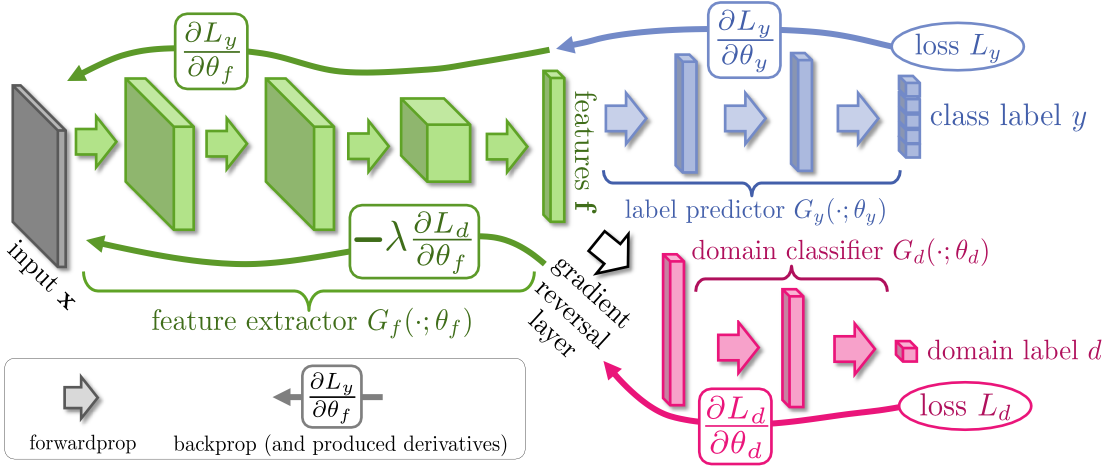
\includegraphics[width=\textwidth]{fig/arch.png}
\caption{Architecture des réseaux adversiaux}
\label{fig:arch}
\end{figure*}

Il reste maintenant à déterminer les hyper-paramètres de notre réseau : 
$\lambda_{D}$, l'architecture du réseau, le pas d'apprentissage, etc.

Puisque l'on ne dispose pas des labels pour les exemples issus du domaine Cible
Il faut trouver un autre moyen pour estimer les performances du modèle.

Ce problème a été abordé dans \cite{Zhong}. La solution proposée, \emph{validation 
inversée croisée} consiste à dire que :

Si le modèle $h$ est performant sur le domaine Cible alors les labels 
prédis sur les données Cibles sont justes. Il est alors possible de s'en servir
pour construire un modèle qui s'adapte dans l'autre sens (du domaine Cible 
vers le domaine Source) et prédire avec précision les labels du domaine Source
que l'on connaît. C'est donc les résultats de ce modèle 'renversé' $h_r$ qui 
indiqueront les performances des hyper-paramètres choisis. 

Tout comme dans le cas de la validation simple, cette méthode peut être 
exécutée sur des découpages différents de l'ensemble des données
afin d'obtenir une estimation plus fine des performances. 
On met de coté une petite partie des données puis on entraîne les deux modèles
($h,h_r$) sur la grande partie restante. Finalement l'évaluation 
s'effectue sur la partie mise de coté.

% subsection méthode (end)


% section le_DANN (end)
\section{Implémentation} % (fold)
\label{sec:implementation}

Dans cette section je vais décrire les choix d'implémentation ainsi que 
quelques détails techniques. Cette section sert surtout à nous rappeler
le pourquoi de certain choix. N'hésitez pas à passer cette section.

Le code est présent ici : \url{https://github.com/victor-estrade/DANN}

Nous avons choisi de ré-implémenter le DANN avec 
\href{http://deeplearning.net/software/theano/}{Theano}
et \href{http://lasagne.readthedocs.org/en/latest/index.html}{Lasagne}
afin de mieux contrôler le code mais aussi pour éviter les problèmes de 
compatibilité entre les versions de \href{http://caffe.berkeleyvision.org/}{Caffe}.

Le workflow de Lasagne fonctionne en 3 temps:
\begin{enumerate}
	\item Définir l'architecture du réseau de neurones
	\item Définir et compiler les fonctions d'entraînement et de test
	\item Entraîner le réseau en lui fournissant les données
\end{enumerate}

\subsection{Les réseaux} % (fold)
\label{sub:les_reseaux}

La première étape est de définir le \emph{Reversal Gradient Layer} (RGL).
Son implémentation ne demande pas trop d'effort mais une certaine connaissance
de Theano et de Lasagne. Cependant le travail a déjà été fait
\href{http://stackoverflow.com/questions/33879736/can-i-selectively-invert-theano-gradients-during-backpropagation}{ici}.

Dans un deuxième temps nous devons définir les réseaux de neurones. Leurs
architectures, la compilation et l'entraînement. Nous avons choisi 
d'implémenter les réseaux sous forme de classe en suivant quelques principes:

\begin{enumerate}
	\item Les données ne doivent pas être un attribut de la classe. Cela 
	facilite la sauvegarde du réseaux et évite que le Garbage Collector ne puisse 
	libérer la mémoire à cause du pointeur présent dans l'objet représentant 
	le réseau de neurone.
	\item La classe ne doit gérer que la partie structure du réseaux de neurone.
	La partie propagation arrière est gérée par les compilateurs afin d'éviter 
	la duplication de code.
	\item Les hyper-paramètres sont donnés au constructeur de la classe autant
	que possible. On évite de séparer les hyper-paramètres. La méthode 
	d'entraînement doit rester simple d'utilisation et ne prendre en argument 
	que les paramètres concernant les données ou le suivi le l'entraînement.
	\item La définition des couches du réseaux se fait dans la méthode 
	\emph{\_build()} appelé en fin d'initialisation. Choix purement esthétique.
	\item La compilation se fait en donnant une fonction de compilation
	gérant la propagation arrière. Une compilation par propagation arrière ie
	une fonction par propagation arrière.
	\item Tous les compilateurs doivent être implémentés de la même façon. 
	Construire les mêmes fonctions, dans le même ordre.
	\item La méthode d'entraînement prend les données en argument et assure le
	suivi de l'entraînement. Elle ne rend rien ou bien elle rend des statistiques
	utiles à l'étude du déroulement de l'entraînement.
\end{enumerate}

Sont implémentés pour l'instant:
\begin{itemize}
	\item Un DANN minimaliste à une seule couche dense de représentation
	\item Un DANN à multiple couche dense de représentation
	\item La descente de gradient stochastique avec ou sans moment.
\end{itemize}

% subsection les_réseaux (end)
\subsection{Quelques détails} % (fold)
\label{sub:quelques_details}

Le code est encore assez mal organisé. Plusieurs refontes sont à prévoir.

Actuellement les données sont transférées sous forme de dictionnaire. Ce qui 
n'est pas nécessairement des plus pratiques. De façon générale la fonction 
d'entraînement n'est pas très bien pensée et changera sûrement à l'avenir.

Lasagne/Theano a comme principal défaut de ne pas permettre d'avoir plusieurs
entrés différentes sur une même couche. Ceci nous oblige à dupliquer les réseaux.
Un réseau correspond à une entrée. Puis il faut forcer le partage des poids afin
de lier la partie commune aux diverses entrées.

Ce problème pourrait être corrigé en utilisant un ConcatLayer qui serait chargé
de concaténer des données d'entrée. Puis un SliceLayer qui ferait le travail inverse
si l'on doit aussi envoyé des sous-parties des données à des sorties différentes.
Cependant le batchsize est pour l'instant donnée au moment de l'entraînement
et non pas à la construction du réseau. Cet utilisation changerait donc la
façon de faire l'entraînement.

% subsection quelques_détails (end)


% section implémentation (end)
\section{Notes} % (fold)
\label{sec:notes}

Ici sont rassemblés les notes, idées et résultats obtenus jusqu'à présent.

\subsection{Rappel personnel} % (fold)
\label{sub:rappel_personnel}

Rappel de cours : les fonctions d'activation comme tanh ou sigmoïde peuvent 
saturer. En général un pas d'apprentissage de l'ordre de 1 est salutaire pour 
pouvoir sortir de l'état saturé. De plus le gradient est borné. Il n'y a donc 
pas de risque de mise à jour trop violente des poids.

Cependant ReLU ne suit pas cette règle. Le gradient n'étant pas borné pour 
cette activation il est recommandé de commencer avec un pas d'apprentissage
faible (de l'ordre de 0.01) afin d'éviter les mises à jour trop violente.

Enfin un pas trop petit pour tanh ou sigmoïde peut être très préjudiciable.
Le gradient serait alors trop petit donc très sensible au bruit.
La descente de gradient reviendrait à demander à une fourmi de trouver la 
vallée dans une route rocailleuse. Elle serait facilement bloquée dans un
minimum local.

Passer de ReLU à tanh ou sigmoïde requiert donc systématiquement d'adapter
le pas d'apprentissage.

% subsection rappel_personnel (end)
\subsection{Reverse gradient layer astuces} % (fold)
\label{sub:reverse_gradient_layer_astuce}

RGL : $\lambda_D = -1 \iff \cancel{\text{RGL}}$

Choisir $\lambda_D = -1$ est équivalent à ne pas avoir de RGL, le gradient se 
retrouve inchangé ($grad \gets -1\times-1\times grad $).

RGL : $\lambda_D = 0 \iff \cancel{\text{Adaptation}}$

Choisir $\lambda_D = 0$ est équivalent à ne pas avoir d'adaptation, le 
gradient se retrouve bloqué par le RGL ($grad \gets -1\times0\times grad $).

En théorie un DANN parfait est un DANN dont la partie classification du
domaine se comporte comme le hasard, la distribution rendant parfaitement
indissociable l'origine des exemples.

Dans la pratique des DANN répondant systèmatiquement le même domaine n'ont 
pas toujours montrés des comportements pathologiques. 
C'est donc au cas par cas ?
En tout cas le visionnage de la matrice de confusion de la sortie "Domaine" du
DANN peut servir et ne coûte pas chère.

% subsection reverse_gradient_layer_astuces (end)
\subsection{Moons} % (fold)
\label{sub:moons}
Commençons pas l'application sur des données artificielles simples et 
facilement interprétables.

L'exemple des 2 lunes imbriquées est un problème non linéaire simple. Un
réseaux de neurone à 1 couche caché de 3 neurones permet de le résoudre
à la perfection.

\begin{figure}[htbp]
\centering
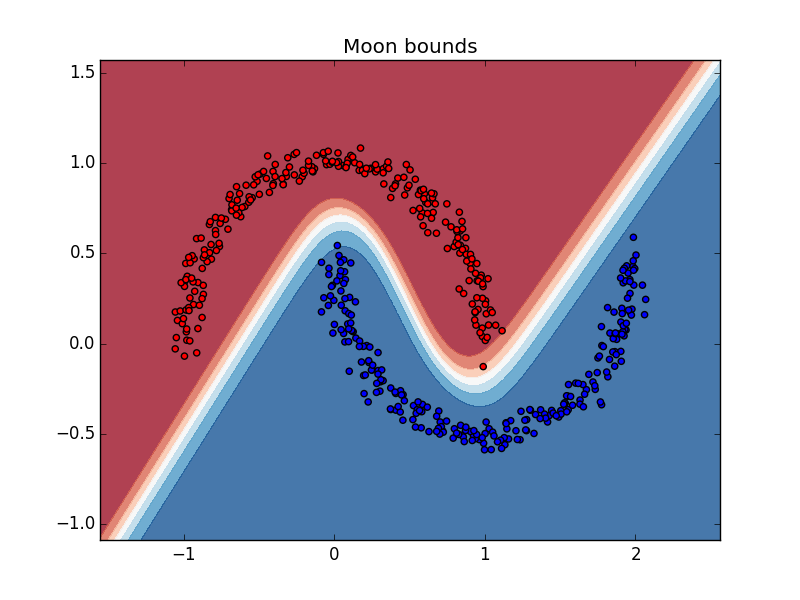
\includegraphics[width=\columnwidth]{fig/moon-bound-0.png}
\caption{Moon classique}
\end{figure}

On peut simuler un problème d'adaptation en appliquant une petite
transformation sur ces données.
Après une rotation de 35 degrés des données le réseau de base perd une bonne
partie de ses performances. On définit donc le domaine Source et Cible
comme étant respectivement les données originelles et les données après
rotation.

L'utilisation d'un \emph{DANN} permet de réduire en partie la perte de 
performance en adaptant le réseau à ces nouvelles données (cf figure \ref{fig:moonrot}.

\begin{figure}[htbp]
\centering
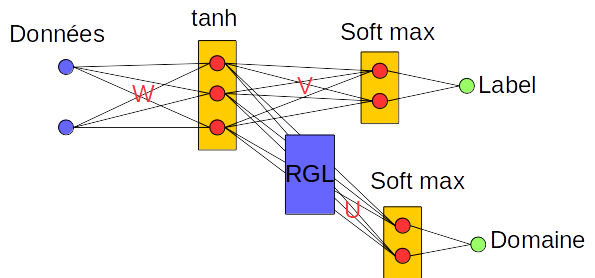
\includegraphics[width=\columnwidth]{fig/DANN-simple.png}
\caption{Structure minimale d'un DANN. (utilisé pour Moon)}
\end{figure}

\begin{figure*}[htbp]
\centering
\subfigure[Sans le DANN les performances sont diminuées.]
	{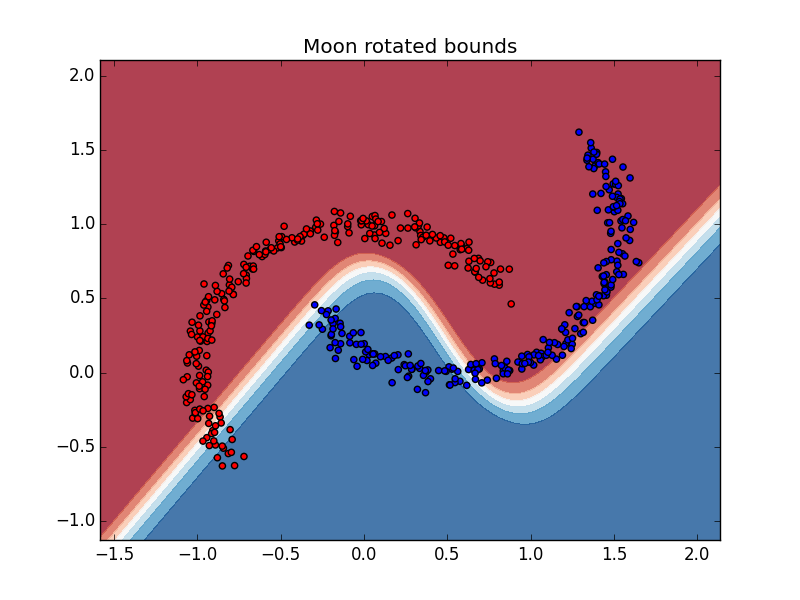
\includegraphics[width=\columnwidth]{fig/moon-rot-bound-0.png}}
\hfill
\subfigure[En appliquant un DANN on peut partiellement corriger ce problème
($\lambda_D=0.7$)]
	{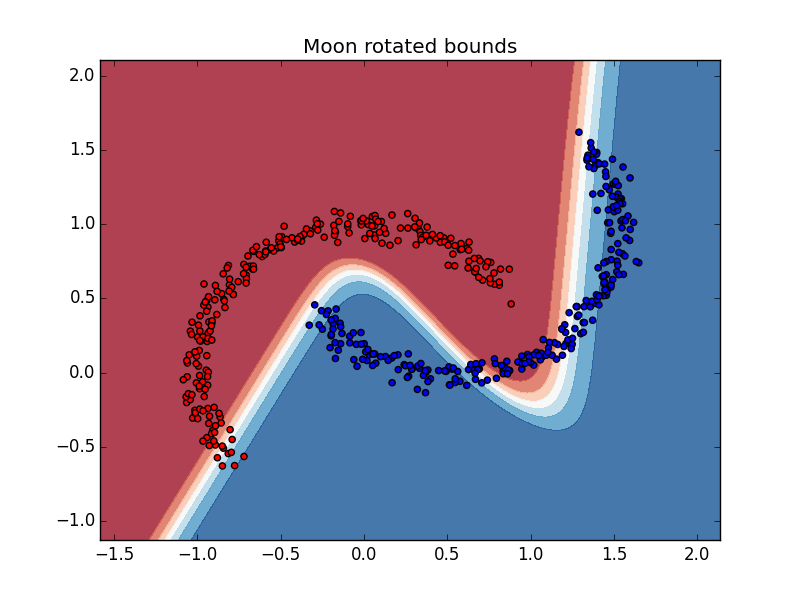
\includegraphics[width=\columnwidth]{fig/moon-rot-bound-1.png}}
\caption{Moon après une rotation de 35 degrés.}
\label{fig:moonrot}

\centering
\subfigure[Avant l'utilisation du DANN.]
	{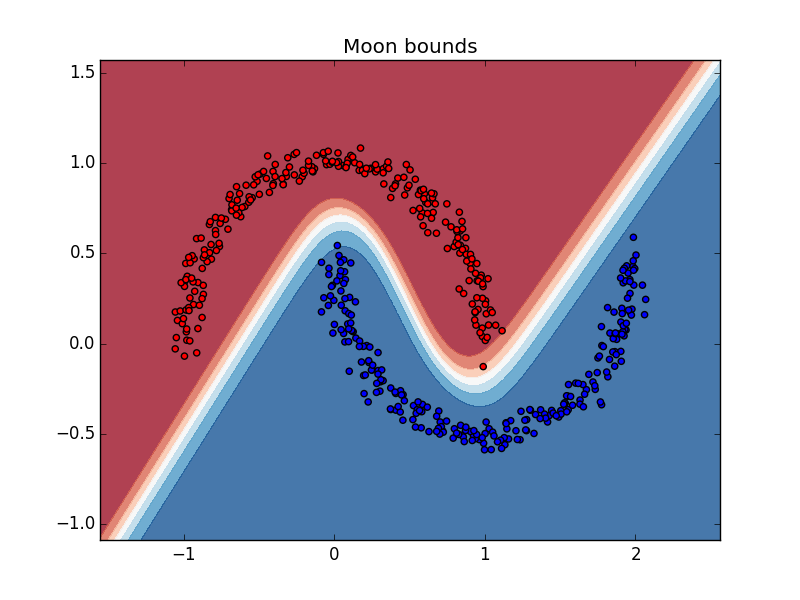
\includegraphics[width=\columnwidth]{fig/moon-bound-0.png}}
\hfill
\subfigure[Le DANN ne fait pas perdre de performances sur ces données.]
	{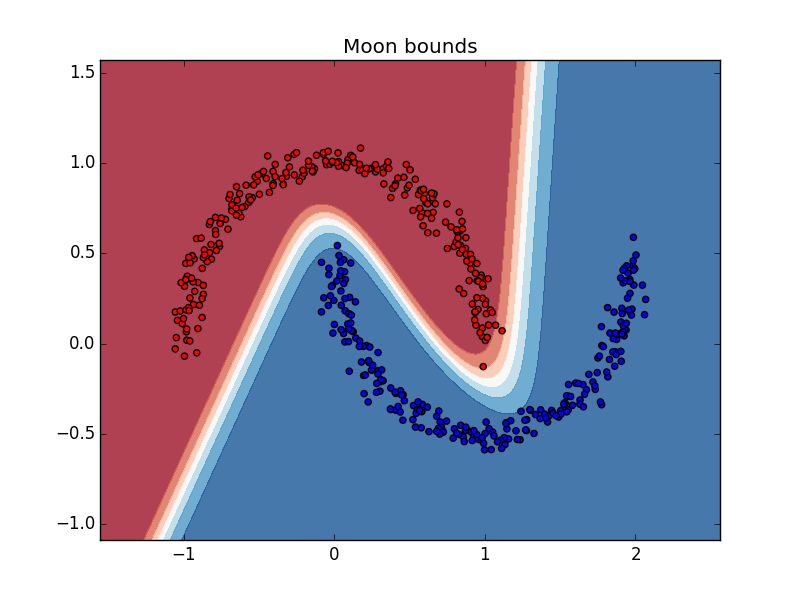
\includegraphics[width=\columnwidth]{fig/moon-bound-1.png}}
\caption{Moon (donnée originale).}
\end{figure*}

Une autre transformation consiste à appliquer une matrice à dominance
diagonale aux données:

$ x \gets A.x $ où $A$ est une matrice à dominance diagonale $(2\times2)$
générée aléatoirement.

On obtient des résultats similaire (cf figure \ref{fig:moonA}).

\begin{figure*}[htbp]
\centering
\subfigure[Sans le DANN.]
	{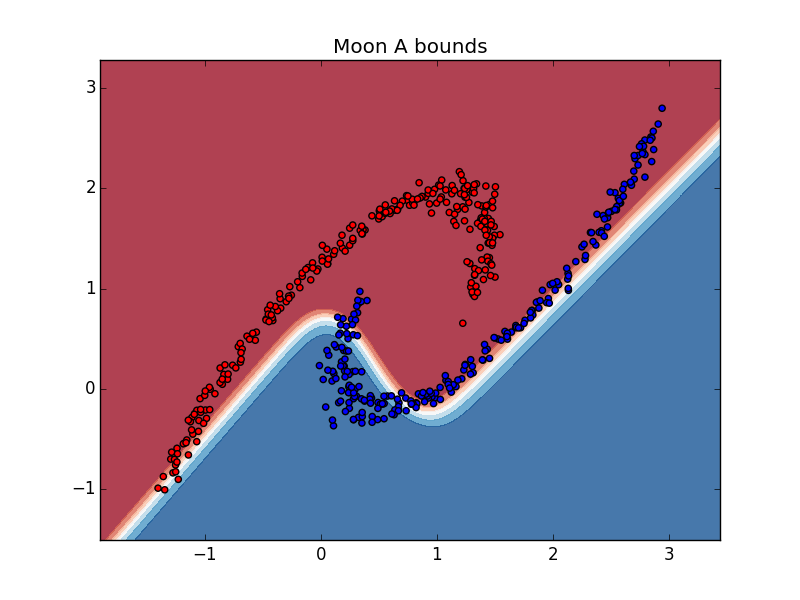
\includegraphics[width=\columnwidth]{fig/moon-A-bound-0.png}}
\hfill
\subfigure[En appliquant un DANN ($\lambda_D=0.7$)]
	{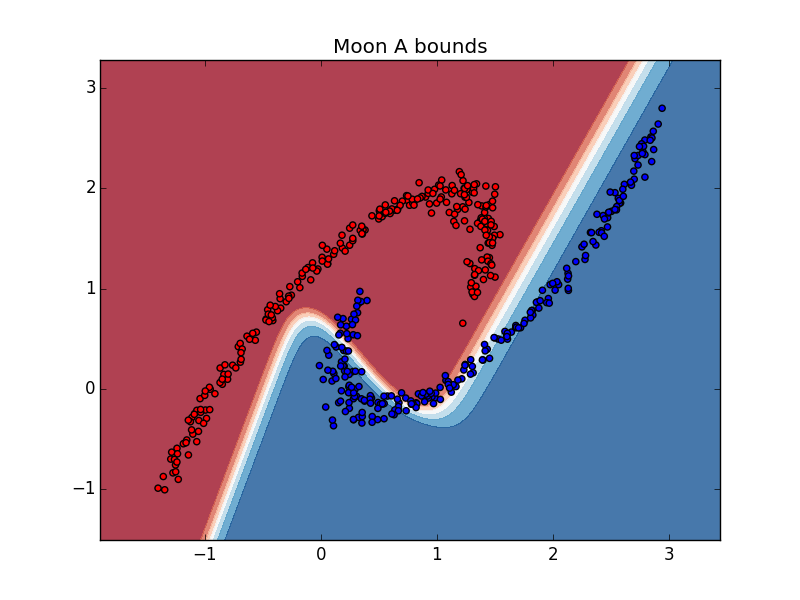
\includegraphics[width=\columnwidth]{fig/moon-A-bound-1.png}}
\caption{Moon après application de $A$.}
\label{fig:moonA}
\end{figure*}


\FloatBarrier
% subsection moons (end)

\subsection{MNIST} % (fold)
\label{sub:mnist}

Étudions maintenant un problème réel à plus grande dimension.
MNIST est le jeu de données le plus classique. Commençons par utiliser la 
transformation en passant par une matrice à dominance diagonale.

$ x \gets A.x $ où $A$ est une matrice à dominance diagonale $(748\times748)$
générée aléatoirement.

Les données ne sont pas grandement modifiées par cette transformation. 
Les changement sont pas visible à l'oeil nu (figure \ref{fig:MNIST-A-sample})

\begin{figure}[htbp]
\centering
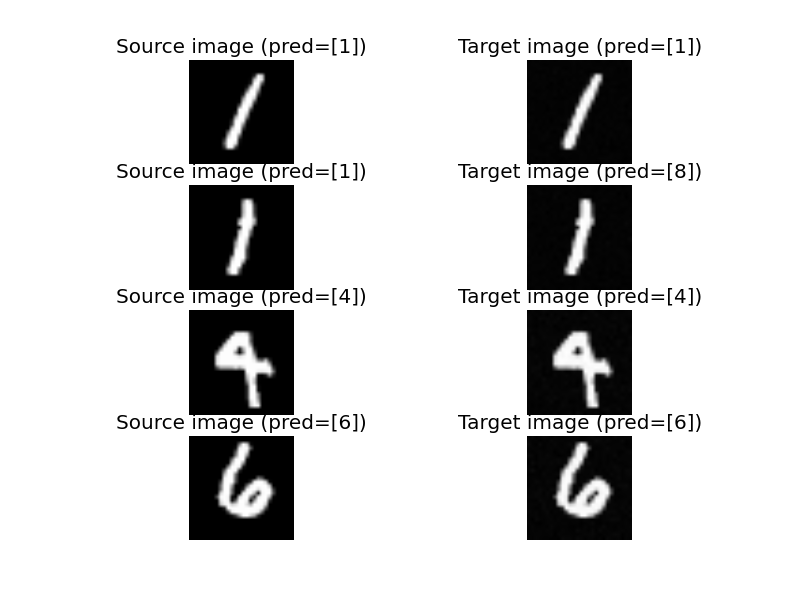
\includegraphics[width=\columnwidth]{fig/MNIST-A-sample.png}
\caption{Examples sur MNIST et MNIST après application d'une matrice à dominance diagonale aléatoire.}
\label{fig:MNIST-A-sample}
\end{figure}

La structure est la même que pour les données \emph{Moons classiques}. 
Un réseaux à une seule couche caché. Cependant la couche cachée compte
maintenant 50 neurones.

Comme on peut le remarquer figure \ref{fig:MNISTA}, le réseaux sans la partie
adaptation fait peu à peu chuter la précision sur les données transformées.
L'utilisation du DANN permet de limiter cette perte de performance.

\begin{figure*}[htbp]
\centering
\subfigure[Sans le DANN.]
	{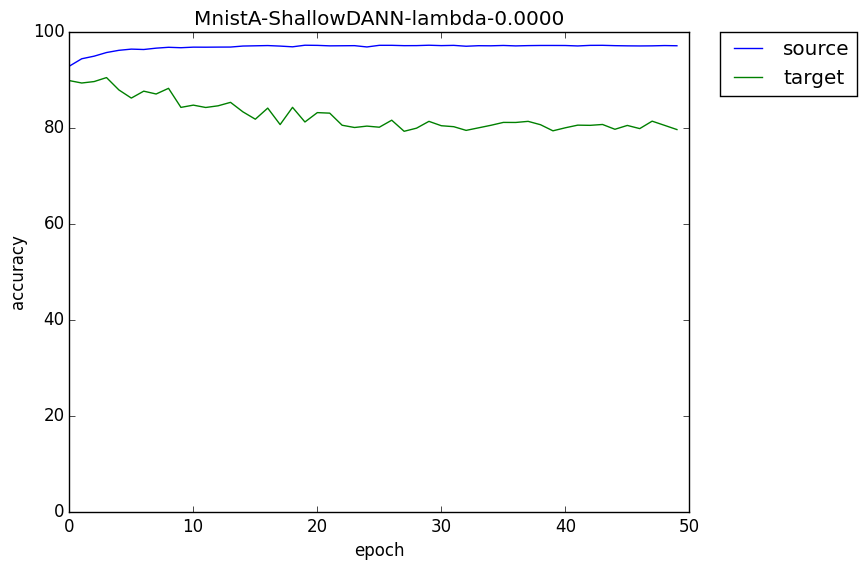
\includegraphics[width=\columnwidth]{fig/MnistA-ShallowDANN-lambda-0.png}}
\hfill
\subfigure[En appliquant un DANN ($\lambda_D=0.01$)]
	{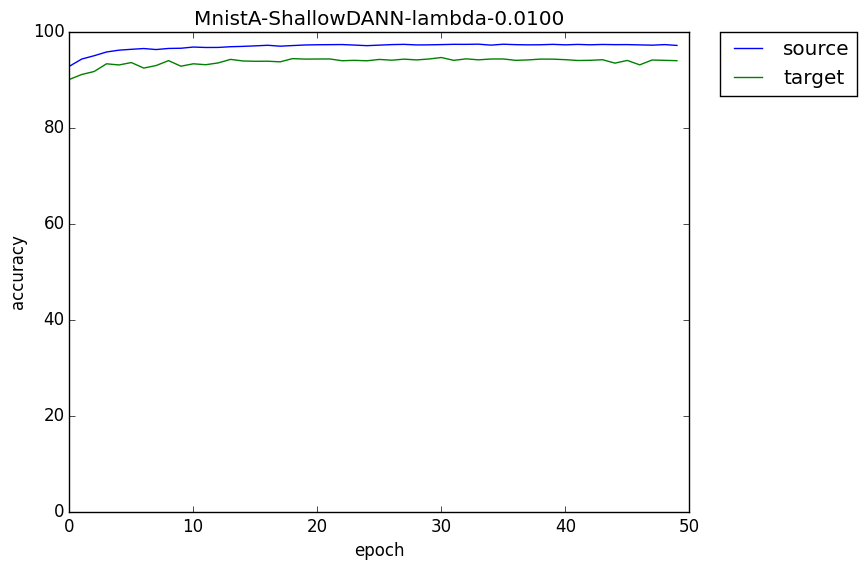
\includegraphics[width=\columnwidth]{fig/MnistA-ShallowDANN-lambda-0,0100.png}}
\caption{Évolution de la précision sur le set de validation sur MNIST et MNIST
	après application d'une matrice à dominance diagonale aléatoire.}
\label{fig:MNISTA}
\end{figure*}

Une autre transformation consiste à appliquer une permutation des pixels.
Dans le cas de MNIST on peut par exemple renverser l'image selon un axe 
(figure \ref{fig:MNIST-Mirror-sample}).

\begin{figure}[htbp]
\centering
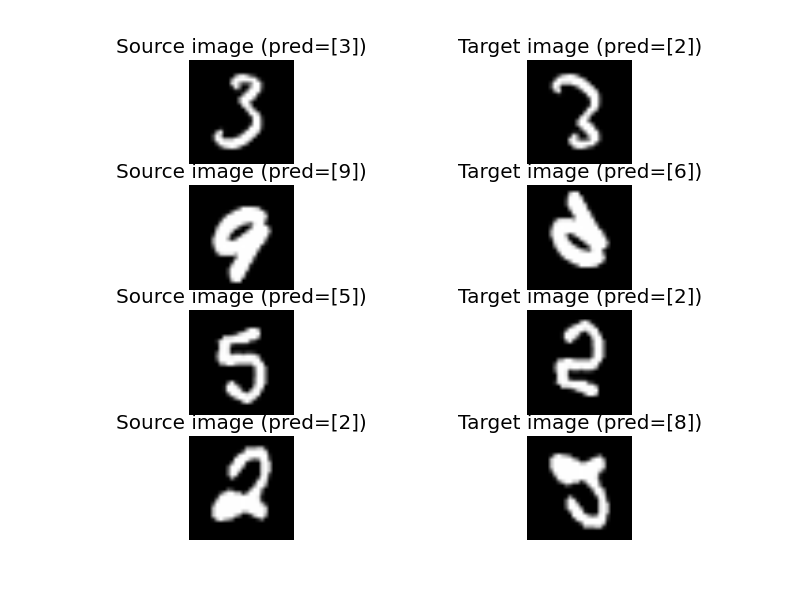
\includegraphics[width=\columnwidth]{fig/MNIST-Mirror-sample.png}
\caption{Examples sur MNIST et MNIST après renversement.}
\label{fig:MNIST-Mirror-sample}
\end{figure}

Cependant cette fois ci le DANN ne semble pas capable de corriger le modèle.
Après avoir essayer diverses configurations et hyper-paramètre j'ai conclu que
la transformation était trop importante pour réussir l'adaptation.

Bien entendu un réseau de neurone avec une couche de convolution règle le 
problème sans même avoir besoin d'adaptation. Mais pour un réseau constitué 
uniquement de couches denses, je n'ai pas obenu de représentation commune 
par entraînement d'un DANN.

Cette fois ci l'architecture utilisée pour la représentation est un peu plus 
complexe : 3 couches denses avec dropout à 50\% et ReLU construite avec 
respectivement 392, 196 et 98 neurones.

Les résultats sont indiqués sous la forme de matrice de confusion figure
\ref{fig:MNIST-Mirror-CM}.

\begin{figure*}[htbp]
\centering
\subfigure[Sans le DANN. $\lambda_D=0$)]
	{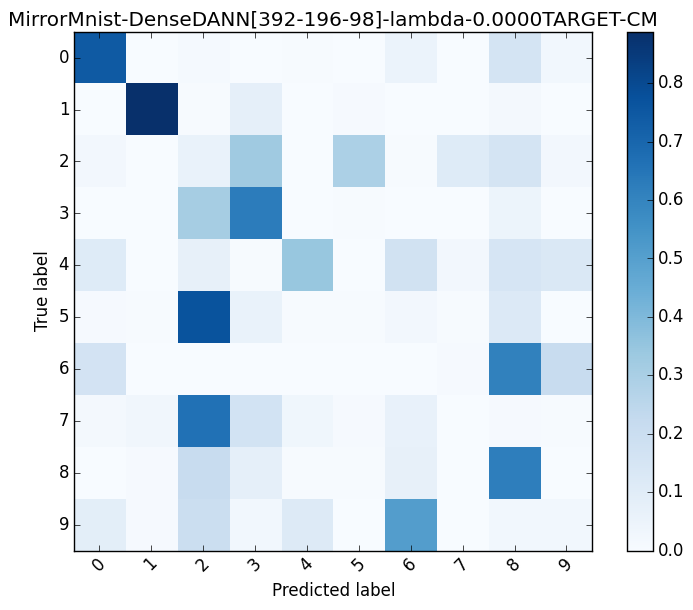
\includegraphics[width=\columnwidth]{fig/MirrorMnist-DenseDANN[392-196-98]-lambda-0,0000TARGET-CM.png}}
\hfill
\subfigure[En appliquant un DANN ($\lambda_D=0.01$)]
	{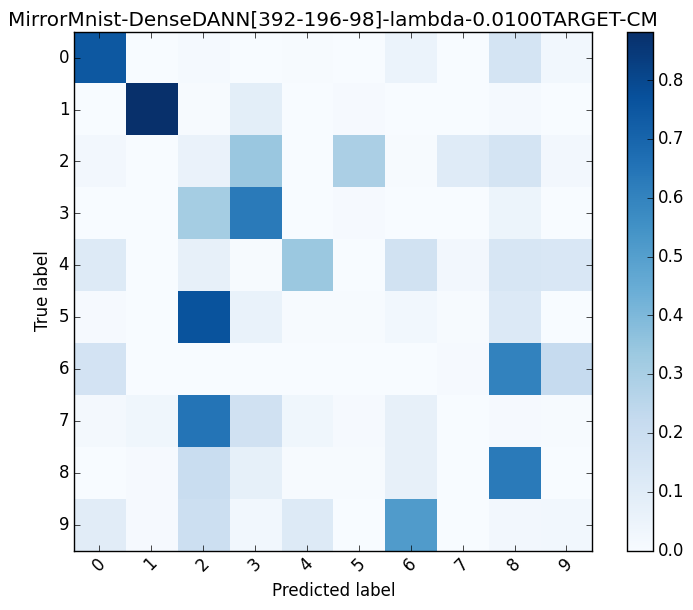
\includegraphics[width=\columnwidth]{fig/MirrorMnist-DenseDANN[392-196-98]-lambda-0,0100TARGET-CM.png}}
\subfigure[Sans le DANN. $\lambda_D=0.1$)]
	{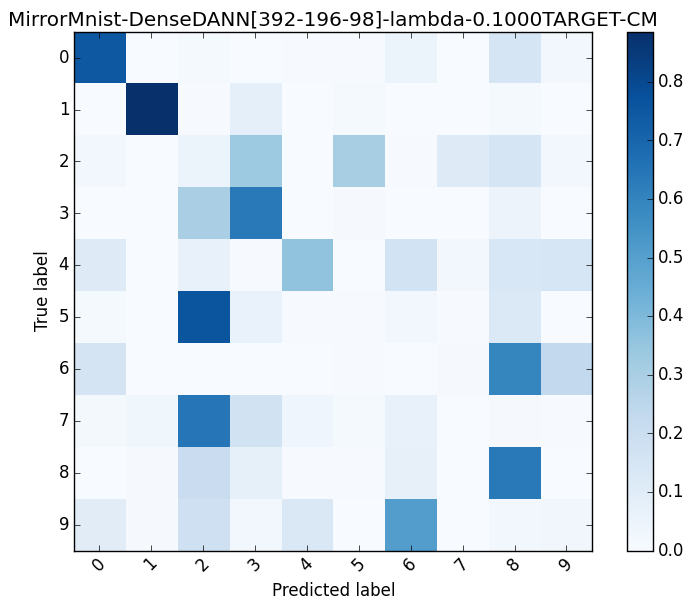
\includegraphics[width=\columnwidth]{fig/MirrorMnist-DenseDANN[392-196-98]-lambda-0,1000TARGET-CM.png}}
\hfill
\subfigure[En appliquant un DANN ($\lambda_D=1.0$)]
	{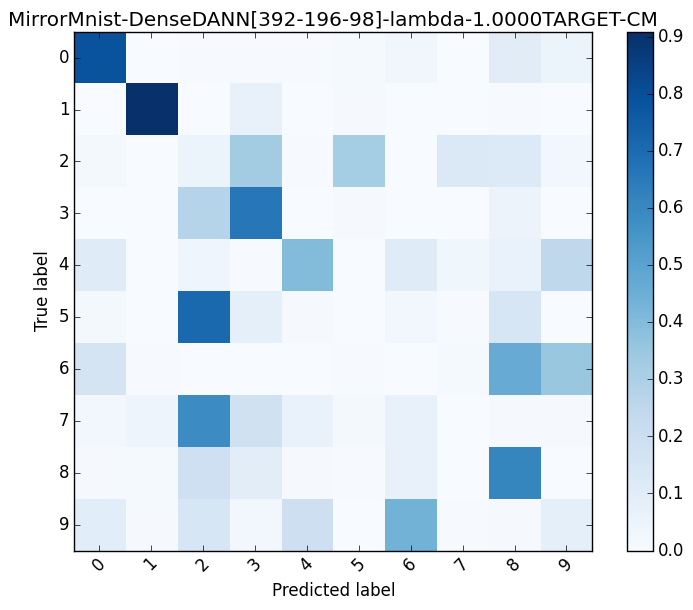
\includegraphics[width=\columnwidth]{fig/MirrorMnist-DenseDANN[392-196-98]-lambda-1,0000TARGET-CM.png}}
\caption{Évolution de la précision sur le set de validation sur MNIST et MNIST
	après application d'une matrice à dominance diagonale aléatoire.}
\label{fig:MNIST-Mirror-CM}
\end{figure*}

% subsection mnist (end)


% section notes (end)
\section{Future} % (fold)
\label{sec:future}

\TODO des tests de l'implémentation
\TODO le clonage des poids pour les réseaux siamois
\TODO passer aux auto-encodeurs

\TODO TSNE
\TODO SVHN vs MNIST régler le problème des tailles d'image par une 
mise à l'échelle
\TODO Implémenter la Reverse (cross) validation
\TODO Grille instead of heat map. Cf Arthur.

\TODO taper dans les données de Higgs ou de robotique


% section future (end)

\bibliography{report}
\bibliographystyle{icml2016}

\end{document} 


% This document was modified from the file originally made available by
% Pat Langley and Andrea Danyluk for ICML-2K. This version was
% created by Lise Getoor and Tobias Scheffer, it was slightly modified  
% from the 2010 version by Thorsten Joachims & Johannes Fuernkranz, 
% slightly modified from the 2009 version by Kiri Wagstaff and 
% Sam Roweis's 2008 version, which is slightly modified from 
% Prasad Tadepalli's 2007 version which is a lightly 
% changed version of the previous year's version by Andrew Moore, 
% which was in turn edited from those of Kristian Kersting and 
% Codrina Lauth. Alex Smola contributed to the algorithmic style files.  
